\section{Anhang}\label{sec:anhang}

\begin{figure}[h]
    \centering
    \begin{minipage}{0.45\linewidth}
        \centering
        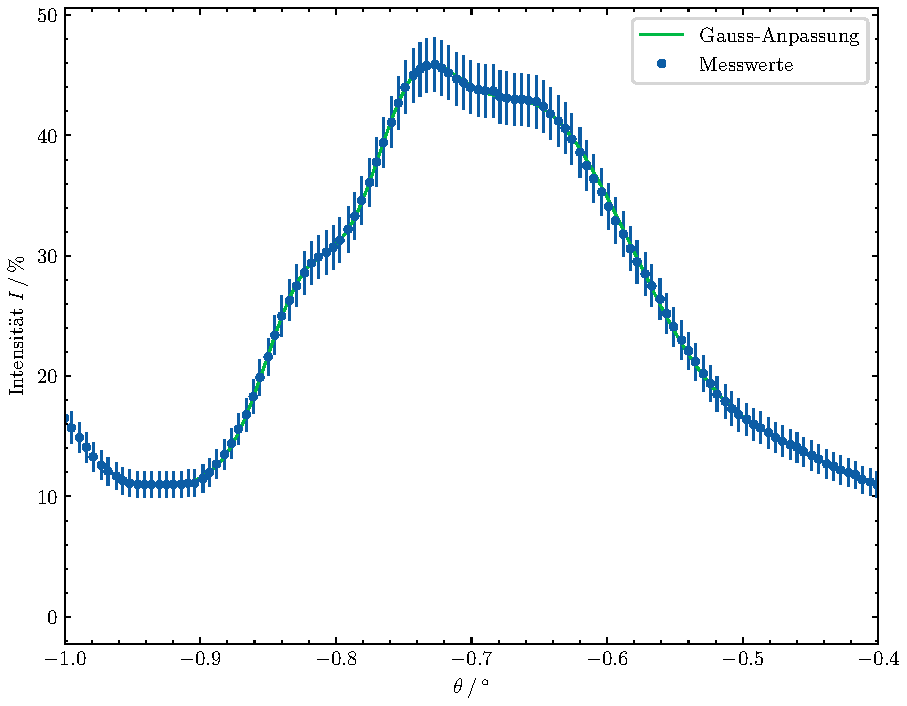
\includegraphics[width=\linewidth]{../figs/gauss_i4.7.pdf}
        \caption{Aufspaltung der Maxima bei \SI{4.7}{\ampere}}
        \label{fig:gauss_i47}
    \end{minipage}
    \hspace{.5cm}
    \begin{minipage}{0.45\linewidth} 
        \centering
        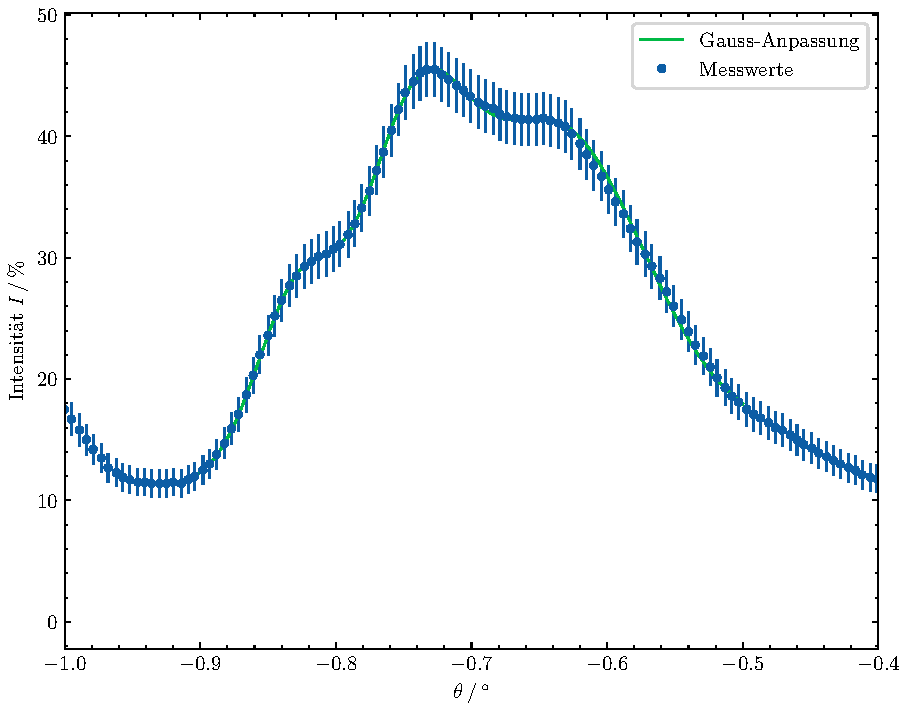
\includegraphics[width=\linewidth]{../figs/gauss_i5.2.pdf}
        \caption{Aufspaltung der Maxima bei \SI{5.2}{\ampere}} 
        \label{fig:gauss_i52}
    \end{minipage}
\end{figure}

\begin{figure}[h]
    \centering
    \begin{minipage}{0.45\linewidth}
        \centering
        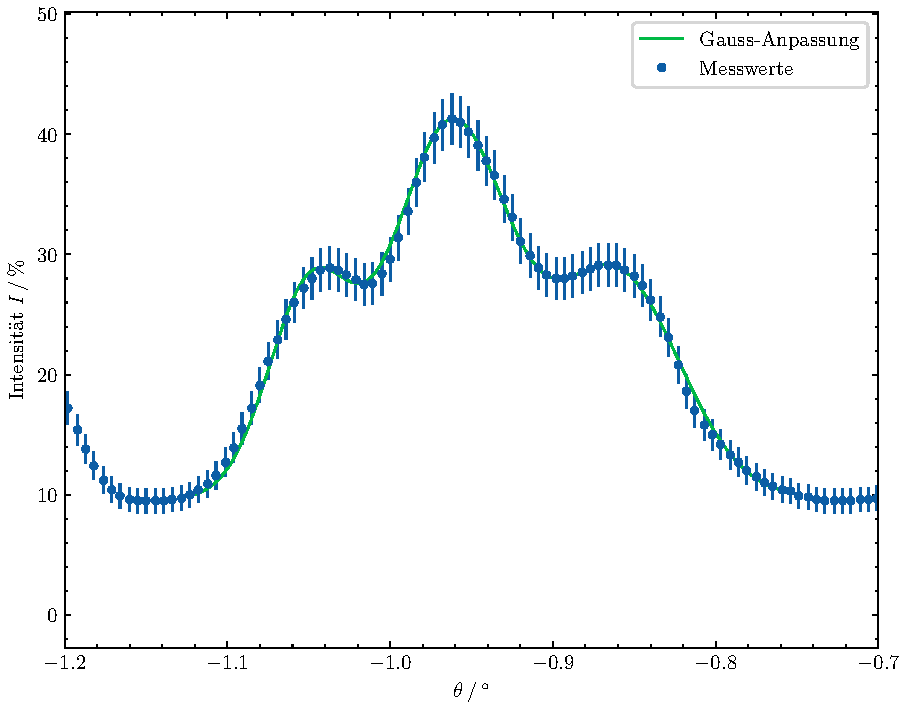
\includegraphics[width=\linewidth]{../figs/gauss_i5.7.pdf}
        \caption{Aufspaltung der Maxima bei \SI{5.7}{\ampere}}
        \label{fig:gauss_i57}
    \end{minipage}
    \hspace{.5cm}
    \begin{minipage}{0.45\linewidth} 
        \centering
        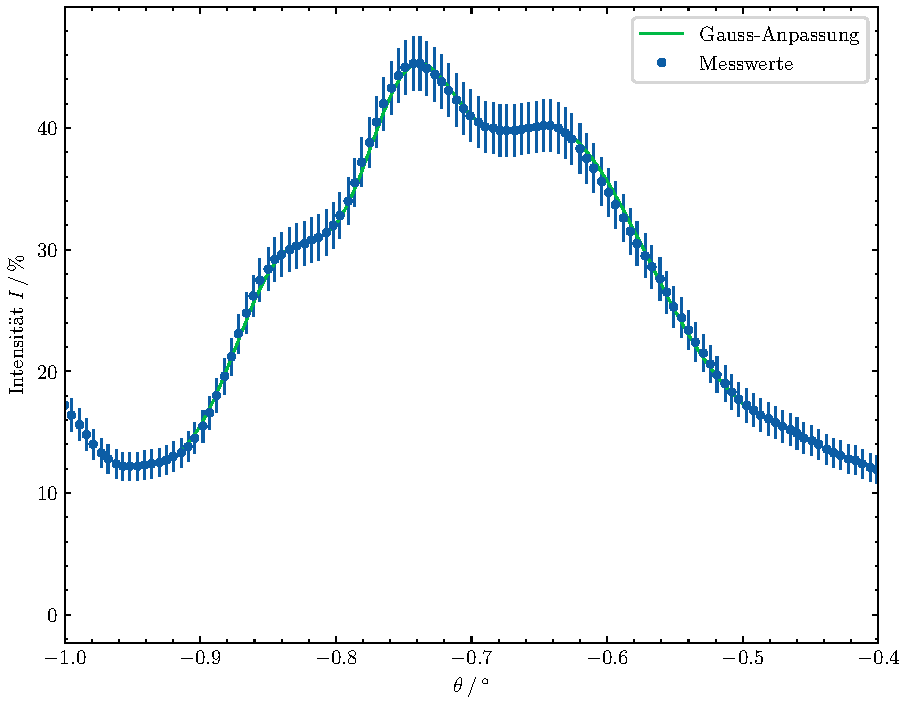
\includegraphics[width=\linewidth]{../figs/gauss_i6.0.pdf}
        \caption{Aufspaltung der Maxima bei \SI{6.0}{\ampere}} 
        \label{fig:gauss_i60}
    \end{minipage}
\end{figure}

\begin{figure}[h]
    \centering
    \begin{minipage}{0.45\linewidth}
        \centering
        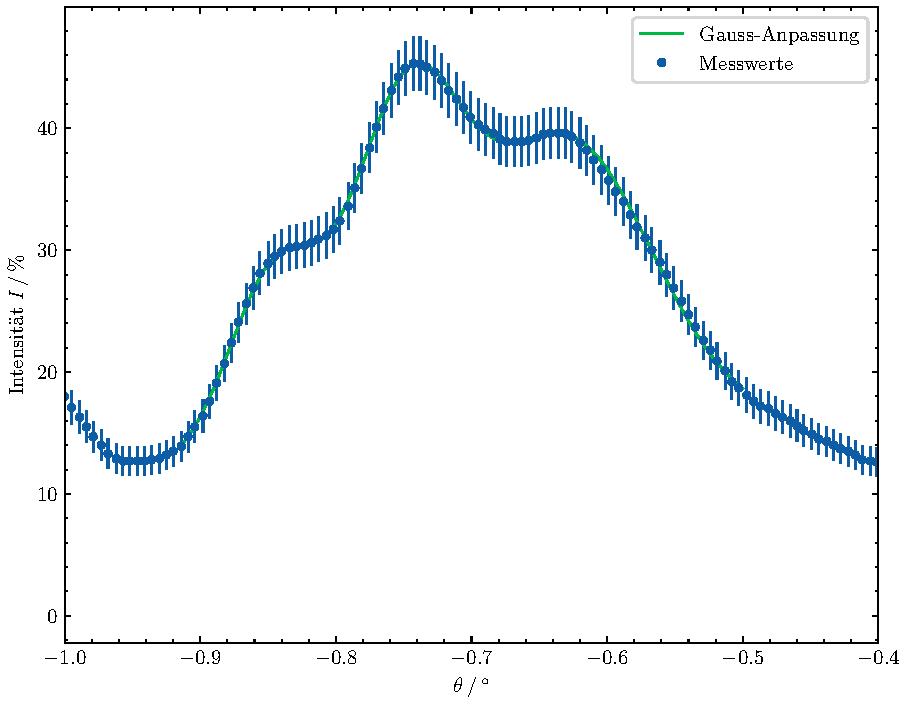
\includegraphics[width=\linewidth]{../figs/gauss_i6.3.pdf}
        \caption{Aufspaltung der Maxima bei \SI{6.3}{\ampere}}
        \label{fig:gauss_i63}
    \end{minipage}
    \hspace{.5cm}
    \begin{minipage}{0.45\linewidth} 
        \centering
        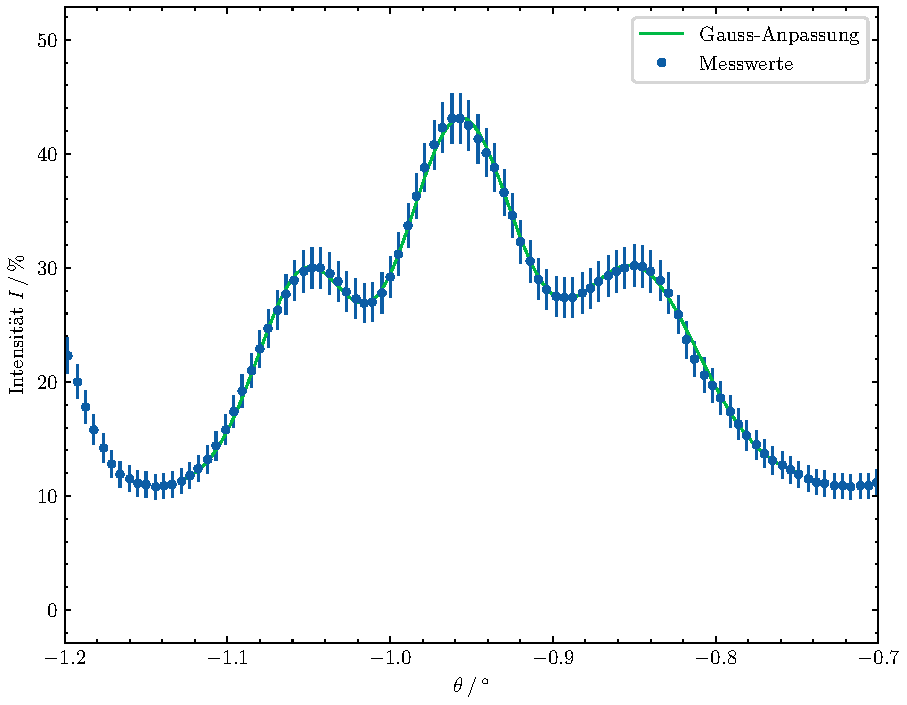
\includegraphics[width=\linewidth]{../figs/gauss_i6.7.pdf}
        \caption{Aufspaltung der Maxima bei \SI{6.7}{\ampere}} 
        \label{fig:gauss_i67}
    \end{minipage}
\end{figure}

\begin{figure}[h]
    \centering
    \begin{minipage}{0.45\linewidth}
        \centering
        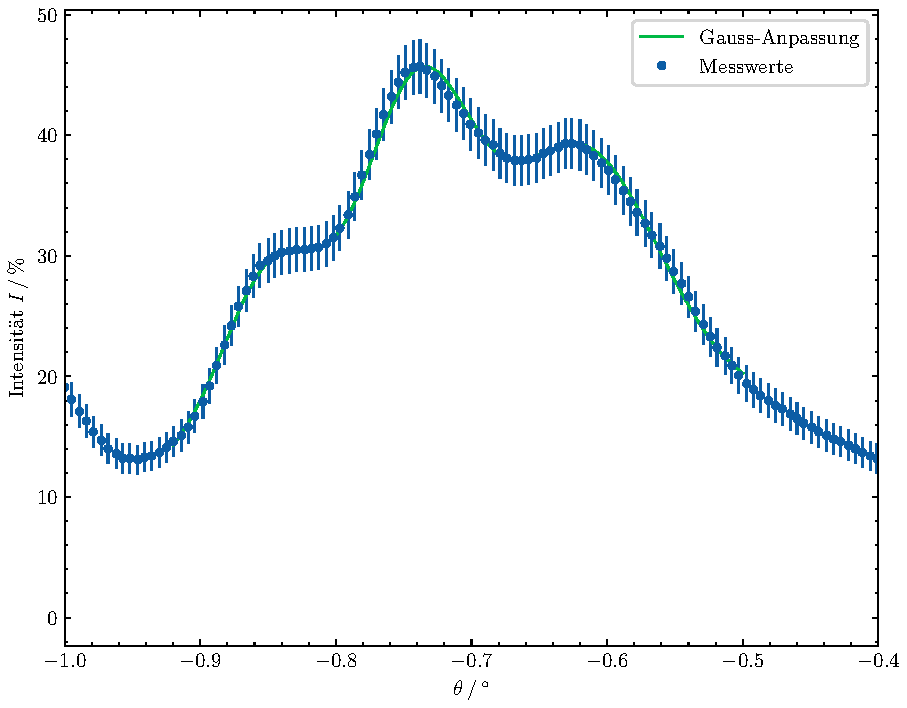
\includegraphics[width=\linewidth]{../figs/gauss_i7.0.pdf}
        \caption{Aufspaltung der Maxima bei \SI{7.0}{\ampere}}
        \label{fig:gauss_i70}
    \end{minipage}
    \hspace{.5cm}
    \begin{minipage}{0.45\linewidth} 
        \centering
        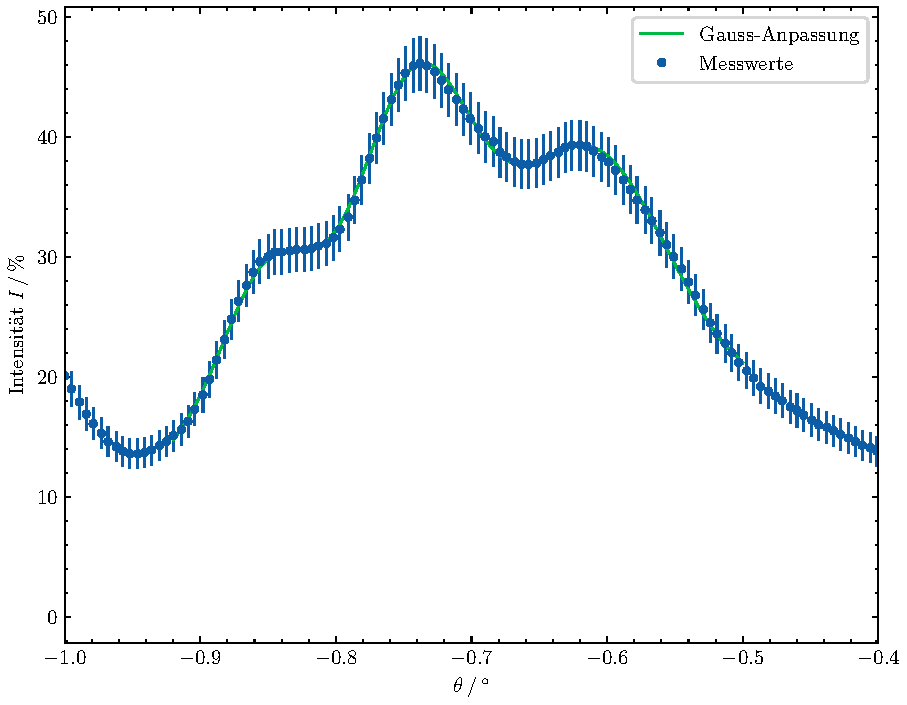
\includegraphics[width=\linewidth]{../figs/gauss_i7.3.pdf}
        \caption{Aufspaltung der Maxima bei \SI{7.3}{\ampere}} 
        \label{fig:gauss_i73}
    \end{minipage}
\end{figure}

\begin{figure}[h]
    \centering
    \begin{minipage}{0.45\linewidth}
        \centering
        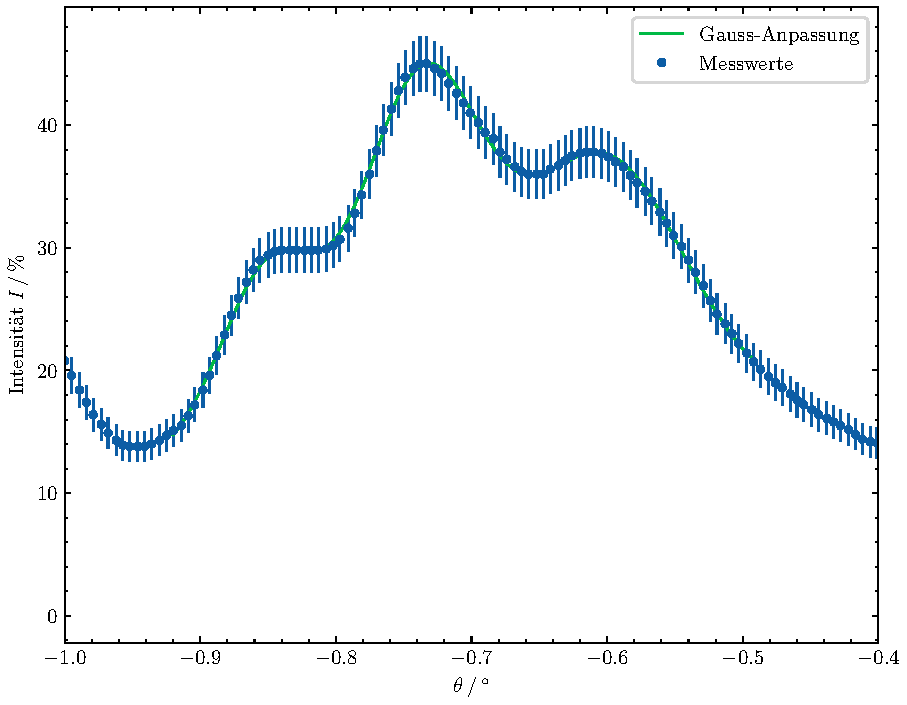
\includegraphics[width=\linewidth]{../figs/gauss_i7.8.pdf}
        \caption{Aufspaltung der Maxima bei \SI{7.8}{\ampere}}
        \label{fig:gauss_i78}
    \end{minipage}

\end{figure}